 

\documentclass{report}
%%%%%%%%%%%%%%%%%%%%%%%%%%%%%%%%%%%%%%%%%%%%%%%%%%%%%%%%%%%%%%%%%%%%%%%%%%%%%%%%%%%%%%%%%%%%%%%%%%%%%%%%%%%%%%%%%%%%%%%%%%%%



\usepackage{epigraph}
\usepackage[toc,page]{appendix}

\usepackage{graphicx}
\usepackage{subfig}


\usepackage{multirow}

\newcommand{\ns}{\noindent }

\newcommand{\sh}[1]{\indent\indent\texttt{\footnotesize\$ #1}}
\newcommand{\shni}[1]{\texttt{\footnotesize\$ #1}}


 \textwidth = 400pt
 \textheight = 570pt
 \oddsidemargin =0 pt

\usepackage[colorlinks=true]{hyperref}



\begin{document}


\begin{titlepage}
    \centering
    \vfill
    {\bfseries\Large
        Toxic Comment Classification challenge\\
         Udacity Capstone - Machine Learning Engineering\\
        \vskip1cm
        R. Angeles\\
    }    
    \vfill
    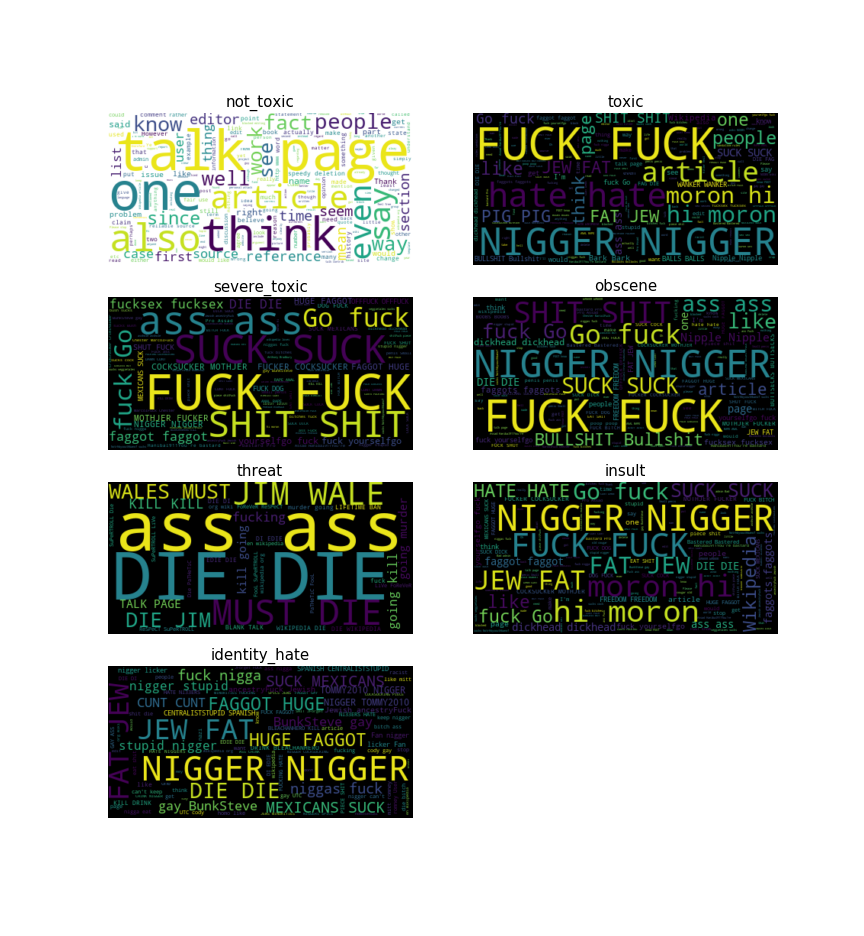
\includegraphics[width=15cm]{../local/plots_tables/clouds.png} % also works with logo.pdf
    \vfill
    \vfill
\end{titlepage}




\chapter{Definition}

\section{Overview}

In this project we work on the Kaggle toxic comment classification challenge that aims improving 
online conversation. In a nutshell, the challenge consist in building an ML model to classify 
Wikipedia, talk edits page, comments as being toxic, severe toxic, obscene, treat or identity hate.


\section{Problem Statement}

Our aim is to explore the performance of three well models for the analysis of
this data set: CNN, GRU and LSTM on top of the GLOVE pre-trained word embedding. 
We not only aimed for a model that performs well but deployed it on website via Sagemaker.

\section{Metrics, goals and reasults}

The benchmark analysis for comparison is the most voted
kernel of the competition: a Naive Bayes - Support Vector Machine model, it reaches 0.9772 auc roc,
while the current leader team reaches 0.98856. The main 
results of the work consist in exploring the performance three popular model for NLP:  CNN, LSTM and GRU.
When combined with a given preprocessing, and using the Glove pretrained word embedding our model 
scores only 0.07\% below 
our benchmark model under 10 mins, on a laptop.

In addition, we deployed the CNN model to an interactive website via SageMaker and on the road 
we create portable utilities to use the benefits Torchtext on Sagemaker pytorch containers. 
After presenting our analysis we discuss performance and future directions. 


\chapter{Analysis}


\section{Data Exploration}

 Jigsaw/Google/Kabble provide a training dataset  of 160K comments, with binary labels
 corresponding to the following classes:
 \emph{Toxic, Severe toxic, Obscene, Threat, Insult or  identity hate}.
 Additionally, a test dataset  with over 153K unlabelled  test comments is provided to make 
 a submission to the competition. The dataset is available at \cite{Kaggle}. This should be placed under a data
 directory to reproduce calculations. Fig.~\ref{fig:train_head} illustrate entries of 
 such dataset. The statistics of this data will be presented below through a series of plots. 
\begin{figure}[!h]
\centering
  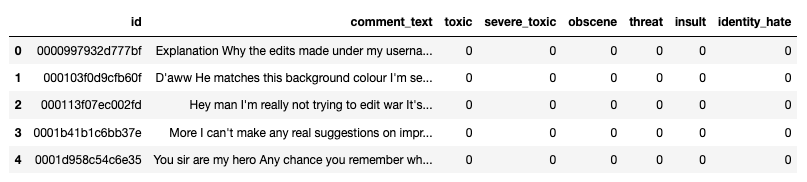
\includegraphics[width=140mm]{../local/plots_tables/train_head.png}
  \caption{Training dataset}
  \label{fig:train_head}
\end{figure}
The most occurrent words corresponding to the labels are in fact shown in the tittle page of this document.


\section{Exploratory Visualisation}


The data exploration is presented on \emph{/local/preprocessing\_exploration.ipynb}. 
The training set is distributed according to Fig.~\ref{fig:bar_plot}. It is extremly imbalanced. 
\begin{figure}[!h]
  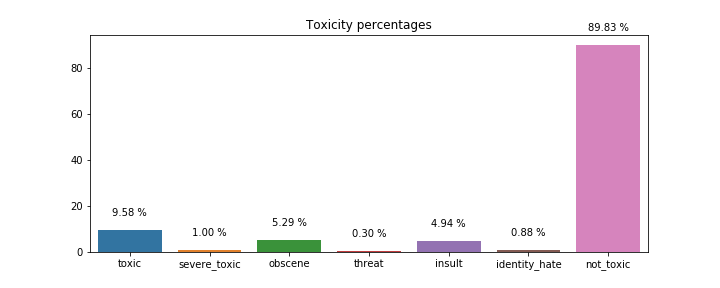
\includegraphics[width=\textwidth]{../local/plots_tables/bar_plot.png}
  \caption{Distribution of the different labels on training set}
  \label{fig:bar_plot}
\end{figure}
Correlations of the labels are shown in Fig.~\ref{fig:corr}
\begin{figure}[!h]
\centering
  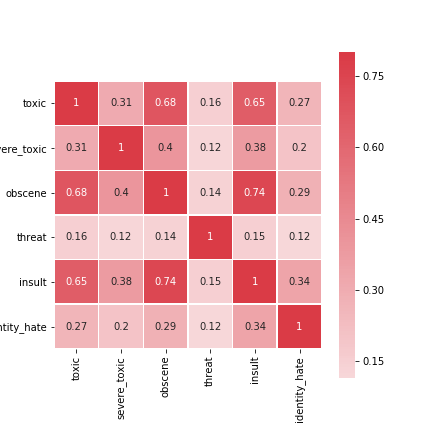
\includegraphics[width=80mm]{../local/plots_tables/corr.png}
  \caption{Correlations coefficients between labels}
  \label{fig:corr}
\end{figure}
Some correlations are large. But since we will predict each class independently this is not a problem. The histogram number of words distribution of the training set comments is presented on Fig.~\ref{fig:hist}. 
\begin{figure}[!h]
\centering
  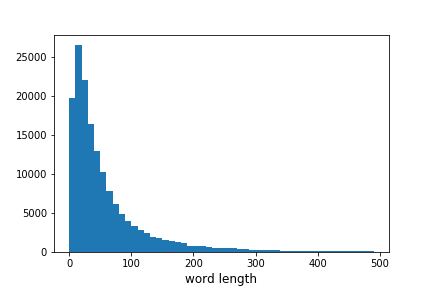
\includegraphics[width=100mm]{../local/plots_tables/word_length_hist.png}
  \caption{Number of words}
  \label{fig:hist}
\end{figure}
There are comments  which are clearly much longer but the vast majority are shorter than 80 words as the cat plots in Fig.~\ref{fig:catplots}.
\begin{figure}[!h]
\centering
  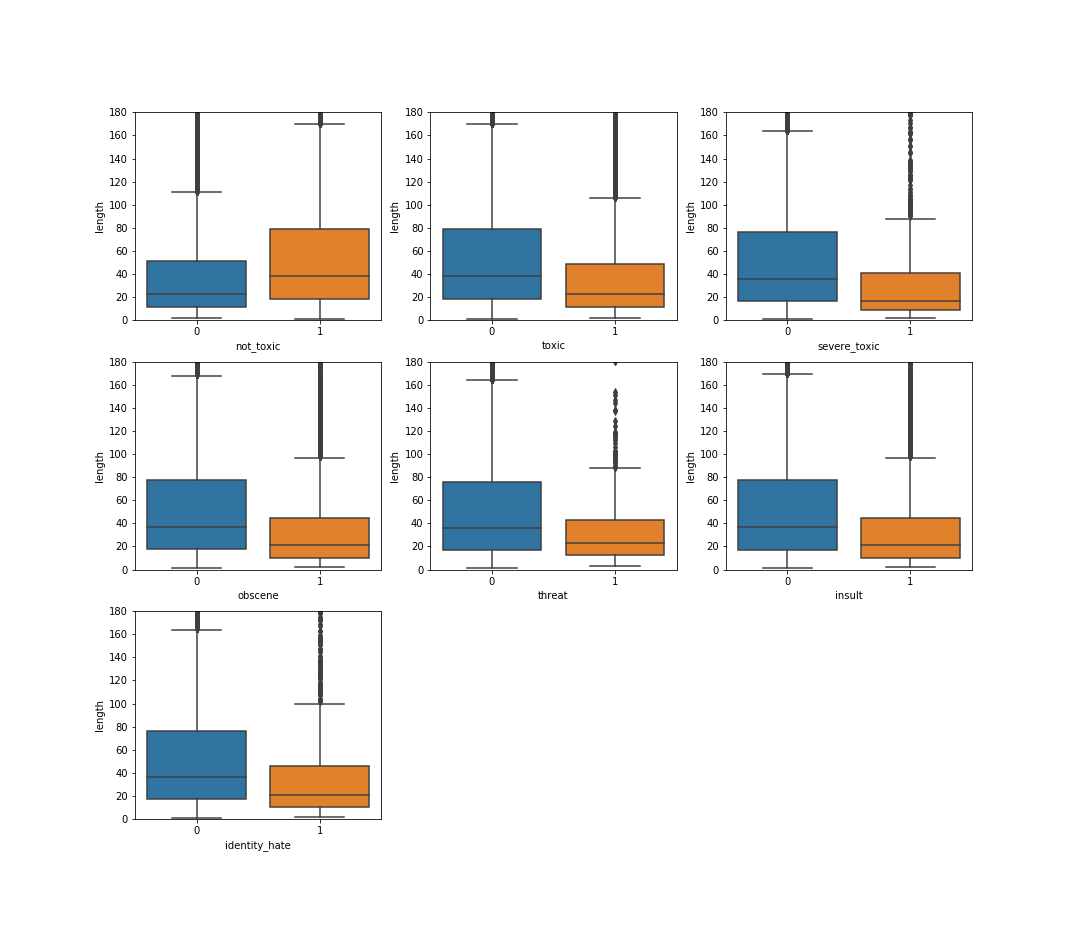
\includegraphics[width=170mm]{../local/plots_tables/catplots.png}
  \caption{Number of words per comment}
  \label{fig:catplots}
\end{figure}

\section{Algorithms and Techniques}

The algorithms used to analyse the text are based 
on dimensional reduce the tokenize representation of words to a pretrained embedding. Specifically, 
we used the word embedding \cite{Glove},
loaded with Torchtext. In order to solve this classification problem,  over this embedding the following deep learning 
architectures applied:
\begin{itemize}
\item Long-Short-Term-Memory.  The foundations of this model can be found at \cite{NG}.
\item Gated-Recurrent-Units.  See \cite{NG} and \cite{Udacity}.
\item Convolutional approach. This scored the best evaluation metric
and was most efficient. An introductory, yet thorough, introduction to this
architecture can be found at Ref.~\cite{BT}.
\end{itemize}
Finally, the model performing the best was deployed to a website via SageMaker. This required creating utilities to make 
torchtext preprocessing objets run on pytorch containers. 

\begin{figure}[!h]
\centering
  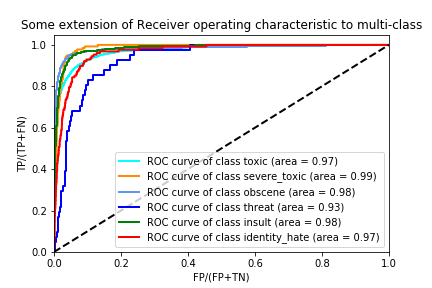
\includegraphics[width=120mm]{../local/plots_tables/rocs.png}
  \caption{ROC curve for the model based on convolutions}
  \label{fig:rocs}
\end{figure}

The last needed technique for the analysis of this work is the 
area under the curve (AUC) of receiver operating characteristic (ROC)
 metric, or rather the average between the different classes. The ROC is defined 
 as the curve generated by plotting the true positive rate  vs the false positive rate 
 for each possible threshold probability value used to predict the classes, and the AUC
 ROC is simply the are under this curve. In fact, since the present problem is a multi-label
 problem the metric is the average AUC ROC obtained for the different classes. 
 
 
 The ROC curves predicted for the convolutional model 
 are presented in Fig.~\ref{fig:rocs}. The AUC ROC is simply the areas under this curves. 
 AUC ROC equal to 1 corresponds to having true positive rate equal to 1 and 
 false positive rate  equal to 0, each probability chosen. As a consequences probability
 predicted for false and positive classes are completely separated. 
 

\chapter{Methodology}

\section{Data Preprocessing}

We three deep learning architectures for natural
language processing. Before applying these, we perform the following 
text preprocessing (found at the local/preprocessing folder if the git repo):
\begin{enumerate}
\item Removed special characters except for numbers and apostrophes, which
were kept according to the english grammar rules.
\item Substitute any numerical character by letter n.
\item Reduce long comments to 80 words. This choice improved our metric 
and it was justified by observing the catplots of Fig.~\ref{fig:hist}. Indeed, 
most comments have 80 or less words. Interestingly most toxic comments tend 
to be shorten than 40 words long.
\end{enumerate}
The next steps were implemented using the \cite{Torchtext} and 
can be found on the /local/building-models folders of the git repo
\begin{enumerate}
 \setcounter{enumi}{3}
\item Stopwords removal was initially implemented but in fact this slightly reduced the
accuracy obtained. 
\item Reducing words to their stemmed also slightly lower our evaluation metric.
\item Tokenization was implemented using the \href{https://scipy.org/scipylib/}{Spicy package}.
\item Comments were fed to models in batches of 256 comments to all models. Comments
 with similar number of words were grouped together, and padded, such that 
each batch had elements with identical number of words. It is worth remarking that this is
easily achieved by Torchtext and that we choose models compatible with this choice. Different 
batches sizes were attempted but such batch size delivered the best evaluation metric performance. 

\item Finally, we embedded the training vocabulary into the 
\href{https://nlp.stanford.edu/projects/glove/}{glove.6B.100d} embedding 
provided by torchtext, with a vocabulary of the 20000 most frequent words on the
training set. Of course plus the unknown and pad tokens, which were set to zero vector before trainig. 
Other vocabulary lends were tried and also the different vocabulary \href{https://fasttext.cc/}{fasttext.en.300d}. 

\end{enumerate}

\subsection{Implementation}

Finally, we trained models on 90\%, randomly chosen, of the training dataset and left the remaining 10\% 
for cross-validation. The following three model architectures were attempted, 
\begin{itemize}
\item Long Short Term Memory (LSTM. We used the 
bidirectional version with hidden dim of 30 for each direction, on top of a dense layer of 30 neurons, 
which were connected to the 6 different classes. Trained for 7 epochs. 

\item Gated Recurrent Unit (GRU) Same configuration 
as LSTM. Trained over 4 epochs. 
\item Convolutional approach. This scored the best evaluation metric
and was most efficient. So we describe it in more detail. In fact, it is a pleasure
to acknowledge credit of this models to the tutorial on sentiment analysis with 
torchtext and pytorch in Ref.~\cite{BT}.
\end{itemize}

The package \emph{PytorchSummaryX} can be use to provide a summary of the model architecture provided 
in Tab.~\ref{fig:cnn}. This table shows that after embeding an input of comments with 15 words each, there are 
three groups of 100 convolution filters acting with dimensions [2,3,4] times 100. This can be tough as examining the 
2 grams, 3 grams and 4 grams to extract features.  There is actually a bug in this program as a max pool layer that acting
on the output convolutions named 1-conv,  2-conv and 3-conv. Such max pool layer outputs a tensor of size 
(batch\_size, (number of convolutions) x (embedding size)). Finally, 
\begin{figure}[!h]
\centering
  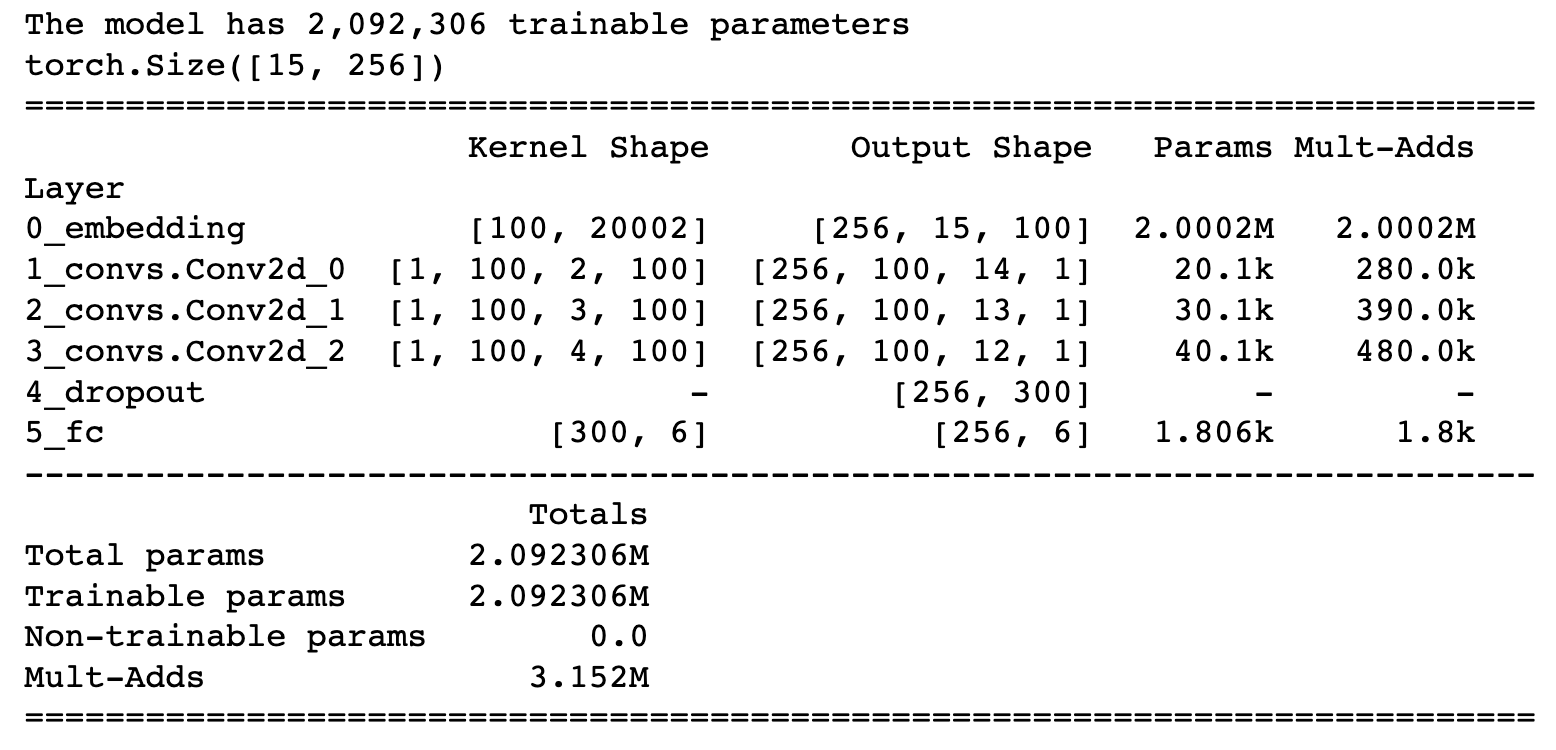
\includegraphics[width=150mm]{../local/plots_tables/cnn.png}
  \caption{NLP based on convolutions}
  \label{fig:cnn}
\end{figure}

This model 2M parameters to train. Most of them correspond to the embedding. This model trained on 9 mins
on a 2017 laptop, and under 4 mins on GPU via SageMaker. Finally it is worth mentioning that in all three cases 
we used dropout regularization, with probability 0.5, for the connected layers.

\section{Refinements}

Some refinements were already mentioned above here we summarize briefly:
\begin{itemize}
\item Tried removing stopwords and stemming words but our models work best by removing all special 
characters and punctuation leaving only aphostrophes. 
\item Boxplots show that the vast mayority of comments are shorter than 80 words so we take this a the word 
limit to analyse. A Future improvement should perhaps break each comment into slices of 80 words. 
\item Used Glove embedding, the best performance was achieved with the 100 dim version tokenizing the 
20,000 most common words appearing on the training data set. Higher numbers seem to reduce accuracy. 
\item The dimension of the dense layer dimension was choosen to run under 1 hour on cpu reaching the highest score. 
\item The number of convolutional filters and its dimensions were also tuned. 
\end{itemize}

\section{Results} 


\subsection{Model Evaluation and Validation}

\begin{figure*}[!t]
\centering
\subfloat{%
  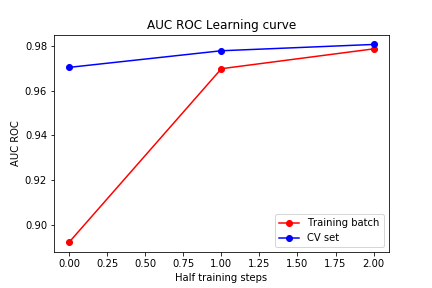
\includegraphics[width=6cm]{../local/plots_tables/AUC_ROC_Learning_curve.png}%
}\qquad
\subfloat{%
  \includegraphics[width=6cm]{../local/plots_tables/Loss_Learning_curve.png}%
}
\\
\subfloat{%
  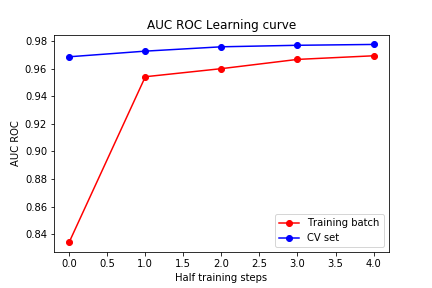
\includegraphics[width=6cm]{../local/plots_tables/lstm_AUC_ROC_Learning_curve.png}%
}\qquad
\subfloat{%
  \includegraphics[width=6cm]{../local/plots_tables/lstm_Loss_Learning_curve.png}%
}
\\
\subfloat{%
  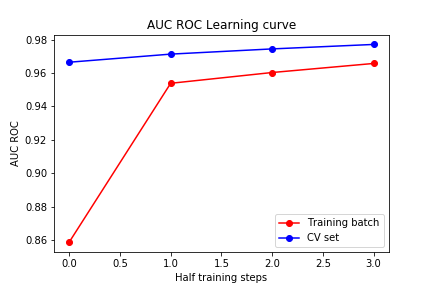
\includegraphics[width=6cm]{../local/plots_tables/gru_AUC_ROC_Learning_curve.png}%
}\qquad
\subfloat{%
  \includegraphics[width=6cm]{../local/plots_tables/gru_Loss_Learning_curve.png}%
}
\caption{Learning curves. The first, second and third rows correspond
to the CNN, LSTM and GRU models respectively. The x axis runs over half epoch steps.}\label{fig:curves}
\end{figure*}

Figs.~\ref{fig:curves} show the learning and loss curves at
half train steps, for the corresponding training batch and over the complete 
cross validation dataset. From each pair of curves one can infer that training is
long enough without overfitting our model to the training set. 


Up to this point it seems like we have solve the problem, reaching the ROC AUC of 
the benchmark model. The final scores rated by kaggle are:
\begin{center}
\begin{tabular}{ |c|c|c|c| } 
\hline
 Model & AUC ROC score on test set\\
 \hline
GRU & 0.9655 \\ 
LSTM & 0.9639 \\ 
NBSVM benchmark&  0.9772 \\ 
CNN & 0.9765\\
Kaggle Leader & 0.9885\\
\hline
\end{tabular}
\end{center}
Two conclusions can form this table. Firstly, our benchmark is a tough competitor as it 
achieves pretty similar results without the complexity of neural networks. Nevertheless, 
we deploy the convolution model to SageMaker reducing the training time to have using a 
ml.xlarge.p2 contained for training. Future work can easily boost the accuracy of our model 
but we leave this as a pending task. Secondly, and more importantly, tables in  
Fig.~\ref{fig:tables}, show that the accuracy other score metrics are not great 
for the extremely imbalanced classes $\{severe\_toxic, threat ,
identity\_hate\}$. 

\begin{figure}[!h]
\centering
  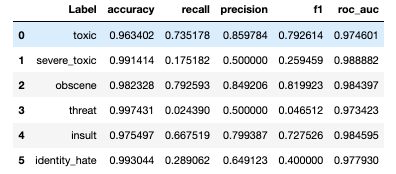
\includegraphics[width=100mm]{../local/plots_tables/cnn_table.png}
\\
\centering
  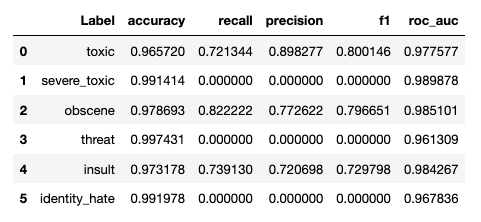
\includegraphics[width=100mm]{../local/plots_tables/lstm_table.png}
\\
\centering
  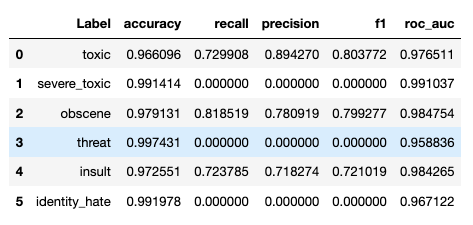
\includegraphics[width=100mm]{../local/plots_tables/gru_table.png}
  \caption{Metric scores. The first, second and third row correspond, respectively, to 
  the best CNN, LSTM and GRU setting found. A probability threshold of 0.5 was set 
  for classifying probabilities into labels.}
  \label{fig:tables}
\end{figure}

Normally, a high AUC ROC would mean that we have a robust model 
whose predicted probabilities for the positive and negative classes 
are well separated. However, the histograms shown in  Fig.~\ref{fig:pdfs},  
for the probability distributions for each fo the true positive and negative classes, show that this is 
not the case for all classes. Clearly, 
for the extremely unbalanced classes more work is need as the probabilities 
for positive and negative classes have a lot of overlapping. 
\begin{figure}[!h]
\centering
  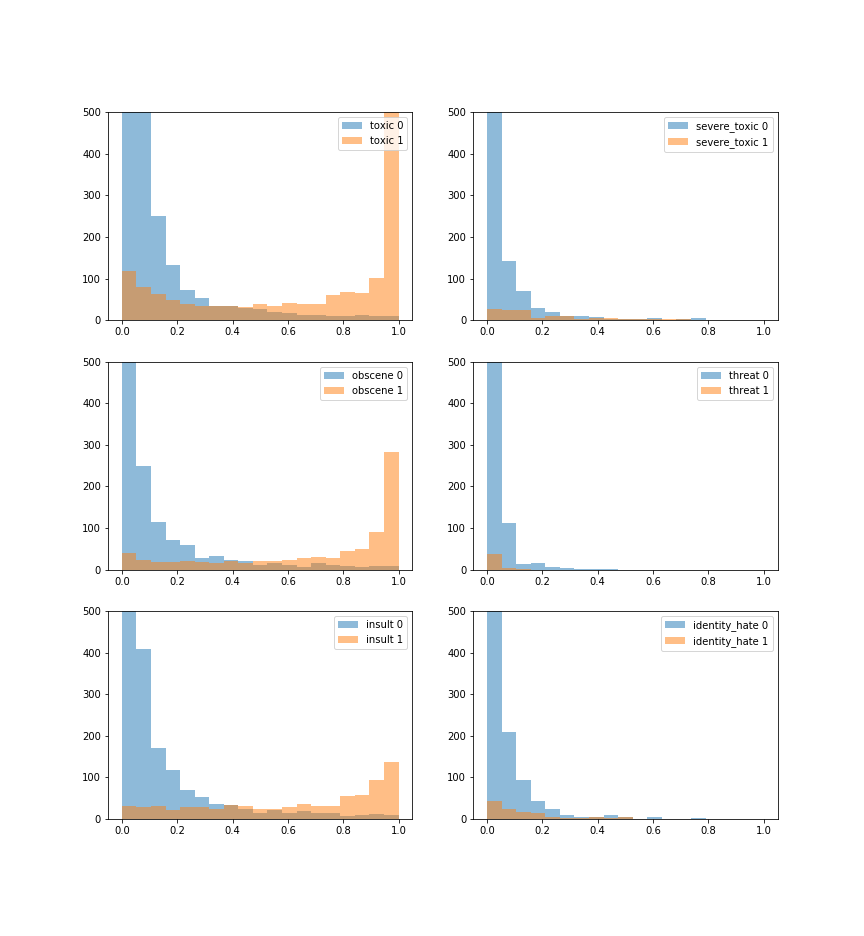
\includegraphics[width=160mm]{../local/plots_tables/pdfs.png}
  \caption{Histograms of predicted probabities for the negative an positve classes. }
  \label{fig:pdfs}
\end{figure}
Future work should address this problem making an Error analysis, addressing imbalance with 
resampling methods or focal loss \cite{focal}. 

\subsection{Justification and deployment}

Our results for for the CNN architecture are comparable to the benchmark, just 0.011\% percent
from the team leading this competition. Furthermore, our model is a good predictor 
has f1 scores above 70\%, on the cross validation datasets for obscene, insults, toxic comments. 
We decided to take this model to SageMaker, retrained there and deploy it to 
the \href{https://reneang17.github.io/The-speech-of-fake-news/}{website}, see Fig.~\ref{fig:website}. 

The deployment of this file involved following similar steps as those presented on \cite{Udacity}. However, 
to use pre-trained embeddings and torchtext (for removing stopwords, stem wods, tokenize, create iterators)
a series of utilities were created. Furthermore, the model is compable to run on GPU significantly reducing 
training time to a half only ml.xlarge.p2 container. All the implementation code for this deployment can be found on
/sagemaker of the github project. I could not find similar utilities form the NLP community so I consider this a valuable
contribution for people using torchtext on SageMaker or those wanting to use TorchText tools on TensorFlow. 


\begin{figure}[!h]
\centering
  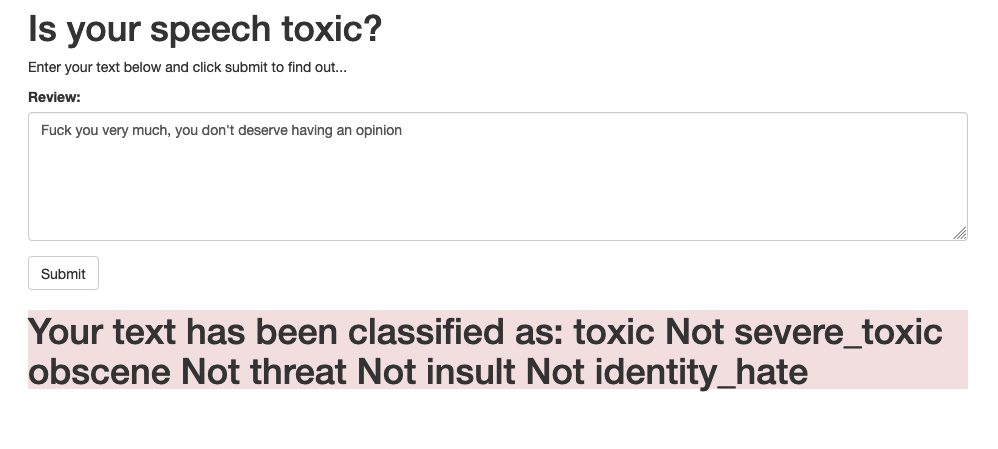
\includegraphics[width=160mm]{../local/plots_tables/website.png}
  \caption{Deployed website}
  \label{fig:website}
\end{figure}



\bibliographystyle{unsrt}
\bibliography{qcd22}

\end{document}
